This chapter briefly summarises the theoretical aspects which lie at the basis of this work. These concepts concern both \gls{dsp} and \gls{dl} fields. On one hand, it is necessary to know the pertinent elements that characterize the reference domain, i.e. digital audio signals. On the other hand, it is important to introduce the main aspects of deep learning models, since they are the main computational systems used for processing audio signals in this project. \\
In order to avoid any unintended confusion or ambiguity, first it is important to say that in this chapter we use a different notation, with respect to the one adopted in the rest of the work, for defining some quantities of interest. This choice is motivated by the fact that notation is determined by the context, which in this chapter is purely theoretical, while in the others is applied to a very specific domain. 

\section{Digital Signal Processing}
The main objective of this paragraph is to present the theoretical fundamentals related to \gls{dsp}. Since the focus is on the audio domain, all the examples deal  mainly with one-dimensional digital signals. \\
Before dealing with \gls{dsp}, we shall briefly introduce a unit of measure which is of fundamental importance for this domain: the Decibel. \\
Formally, \gls{db}is a logarithmic measure that evaluates the ratio between two homogeneous quantities (two powers, two energies, etc$\dots$). The formula for expressing a ratio $Q$ in \gls{db} is as follows:
\begin{align}
	Q (dB) = 10 \log_{10}(Q)
\end{align}
where $Q$ is a ratio between two homogeneous quantities (which share the same unit of measure). \\
\subsection{Classification of Signals}
Signals can be categorized according to various criteria: \textit{multi-channel} vs \textit{single-channel}, \textit{real-valued} vs \textit{complex-valued}, \textit{one-dimensional} vs \textit{multi-dimensional}, \textit{continuous-valued} vs \textit{discrete-valued}. It is important to define such a categorization because some techniques can only be applied to specific families of signals. The objective of this paragraph is to outline in a comprehensible and exhaustive way the main families of signals. \\
As mentioned in Chapter~\ref{chap:intro}, it is possible to define a signal $x$ as a function of one or more independent variables. Formally, we can consider $x:\mathcal{A} \rightarrow \mathcal{B}$ where $\mathcal{A}$ and $\mathcal{B}$ are subsets of real vector spaces of dimension $\mathbb{R}^m$. The values of the domain $\mathcal{A}$ usually refer to spatial and/or temporal coordinates, while the codomain $\mathcal{B}$ denotes values assumed by physical quantities such as pressure, currents. For example, audio signals such as speech and music concern variations of air pressure over time. \\
According to \cite{proakis2006dimitris}, we can consider different families of signals, depending on whether or not their domain and codomain vector spaces are real: a first distinction can be made between “continuous-time” and “discrete-time” signals. \\
Continuous-time ones are defined for every value of time, so they take on values over the interval $(-\infty, \infty)$. The functions $x_{1}(t)=\cos \pi t, x_{2}(t)=e^{-|t|}$ $-\infty<t<\infty$ are good examples of this class of signals. \\
On the other hand, we have functions which are defined only at discrete instants of time, i.e. discrete-time signals. They may arise by a sampling process that takes place over \textit{analog} signals at discrete time instants. The main factors that characterize the sampling operation are discussed in more detail in \ref{from_a_to_d}. In many practical applications, discrete-time signals are obtained by a periodically sampling of analog signals, such that time instants are equidistant. The signal $x\left(t_{n}\right)=e^{-\left|t_{n}\right|}, n=0,\pm 1,\pm 2, \ldots$ is an example of a discrete-time signal. For the rest of the work, we use the index $n$ to emphasize the discrete-time nature of a signal as $x(n)$ instead of $x(t)$. \\
Furthermore, values in the codomain $\mathcal{B}$ can be either continuous or discrete. In particular, if a signal takes on all possible values on a certain range, it is said to be a continuous-valued signal. Alternatively, if the signal is obtained by quantizing its values to a finite set of discrete values, it is said to be a discrete-valued signal. \\ 
In summary, it is possible to distinguish the following classes of signals:
\begin{itemize}
	\item $\mathcal{A}\in\mathbb{R}$, $\mathcal{B}\in\mathbb{R}:$ continuous-time and continuous-valued signals, also known as \textit{analog} signals;
	\item $\mathcal{A}\in\mathbb{R}$, $\mathcal{B}\in\mathbb{Z}:$ \textit{quantized analog} signals, i.e. continuous-time and discrete-valued signals;
	\item $\mathcal{A}\in\mathbb{Z}$, $\mathcal{B}\in\mathbb{R}:$ discrete-time and continuous-valued signals, also known as \textit{sampled} signals;
	\item $\mathcal{A}\in\mathbb{Z}$, $\mathcal{B}\in\mathbb{Z}:$ \textit{digital} signals, i.e. discrete-time signals having a set of discrete values. In this work we only deal with digital signals since they are the only ones that can be processed by a computer.
\end{itemize}
It is important to mention that, for simplicity of notation, in the above definitions we refer to the discrete set of values with the integer symbol $\mathbb{Z}$. A graphical example of this categorization is provided in Figure ~\ref{fig:signals}.

\begin{figure}[H]
	\begin{center}
		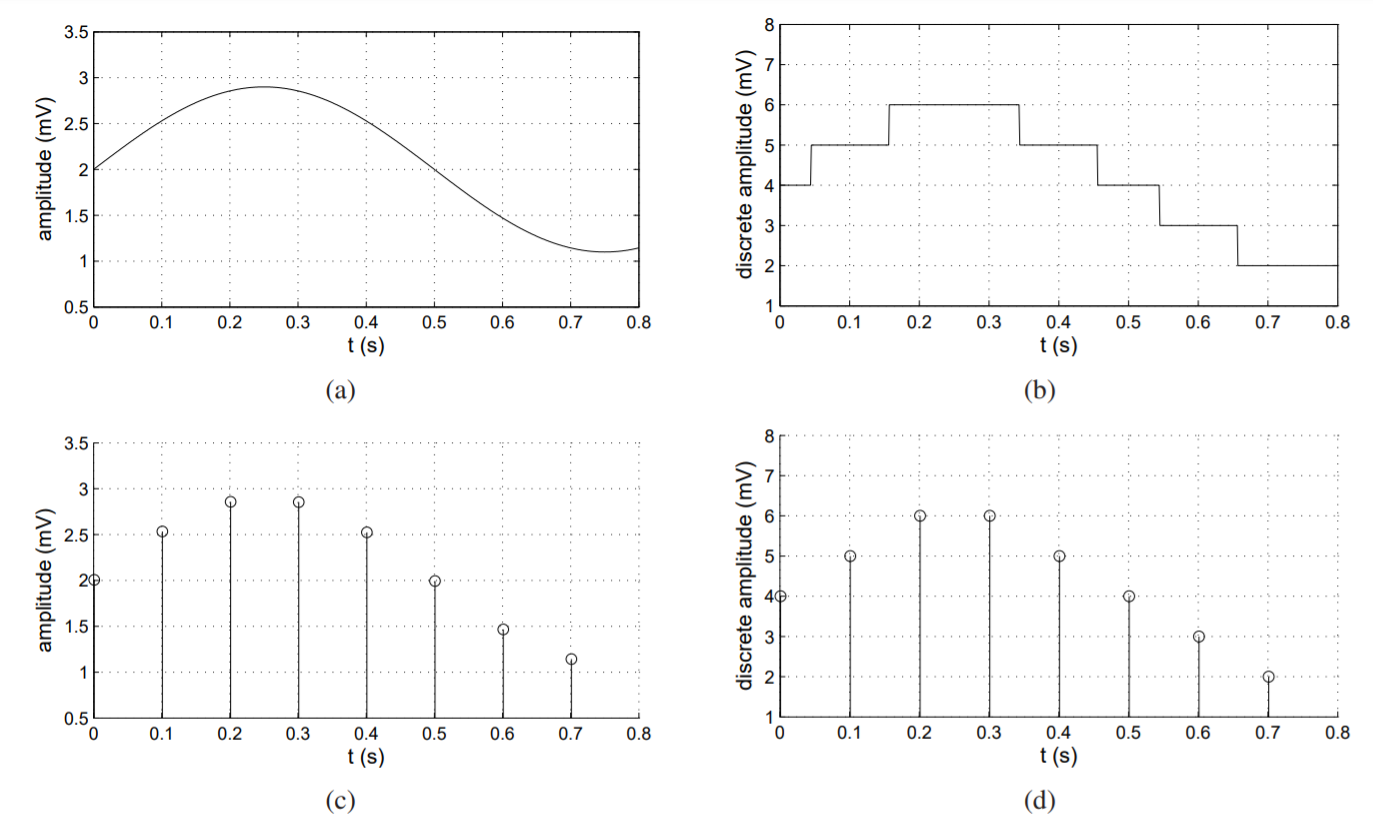
\includegraphics[scale=0.57]{img/signals.png}
		\captionsetup{margin=2cm}
		\caption{ (a) \textit{Analog}, (b) \textit{quantized-analog}, (c) \textit{sampled}, and (d) \textit{digital} signals. From \cite{avanzini2005fundamentals}.} 
		\label{fig:signals}
	\end{center}
\end{figure}
\noindent Furthermore, we can distinguish \textit{one-dimensional} and \textit{multi-dimensional} signals depending on the vector space dimension of $\mathcal{A}$. In particular, a signal is called one-dimensional if its value is a function of a single independent variable. An example of this class of signals is the audio, which is function of time. On the other hand, if the signal is a function of M independent variables, the signal is called a M-dimensional one. For example, images are function of two spatial coordinates. \\
Another distinction can be made between \textit{single-channel} and \textit{multi-channel} signals. Examples of the former category are mono recordings or black and white images, while stereo audio clips and RGB digital images are examples of the latter. In this thesis project we work mainly on single-channel, one-dimensional signals.

\subsection{From Analog to Digital} \label{from_a_to_d}
As previously motivated, this work deal mainly with digital signals. That means they are a sequence of data bits, obtained through a process that allows to convert signals from their original analog form to a digital one. According to \cite{proakis2006dimitris}, this procedure is called \gls{ad} conversion, and the corresponding devices are called \gls{ad} converters. \\
It is possible to divide this process into three main steps:
\begin{enumerate}
	\item \textit{Sampling}. This is the conversion of a continuous-time signal into a discrete-time one.
	\item \textit{Quantization}. It is basically an approximation process that consists in converting a continuous-valued signal into a discrete-valued one.
	\item \textit{Coding}. In this process, each discrete value is represented by a b-bit binary sequence.
\end{enumerate}
This section aims to deepen these three steps, since they are fundamental in plenty of \gls{dsp} applications. The main reference for this explanation is \cite{proakis2006dimitris}. \\
As previously mentioned, sampling is the first step of the \gls{ad} conversion.
This can be done in many ways, but in many practical applications a discrete-time signal $x(n)$ is obtained by a \textit{periodic}
or \textit{uniform} sampling of analog signals. If we denote with $x_{a}(t), \quad-\infty<n<\infty$ the analog signal, then the discrete-time signal can be calculated as follows:
\begin{align}\label{eq:from_a_to_d}
	\begin{array}{c}
		x(n)=x_{a}(nT), \quad-\infty<n<\infty
	\end{array}
\end{align}
\noindent where $T$ are the seconds between successive samples. This time interval $T$ is called the \textit{sampling period} or \textit{sample interval} and its reciprocal $1 / T=F_{s}$ is called the \textit{sampling rate} (samples per second) or the \textit{sampling frequency}, that is commonly measured in \gls{hz} (cycles per second). Equation \ref{eq:from_a_to_d} establishes a linear relationship between the time variables $t$ and $n$, that can be expressed as:
\begin{equation}\label{eq:tn_relation}
	t=n T=\frac{n}{F_{s}}
\end{equation}
\noindent A graphical example of the periodic sampling is given in Figure \ref{fig:periodic_sampling}.
\begin{figure}[H]
	\begin{center}
		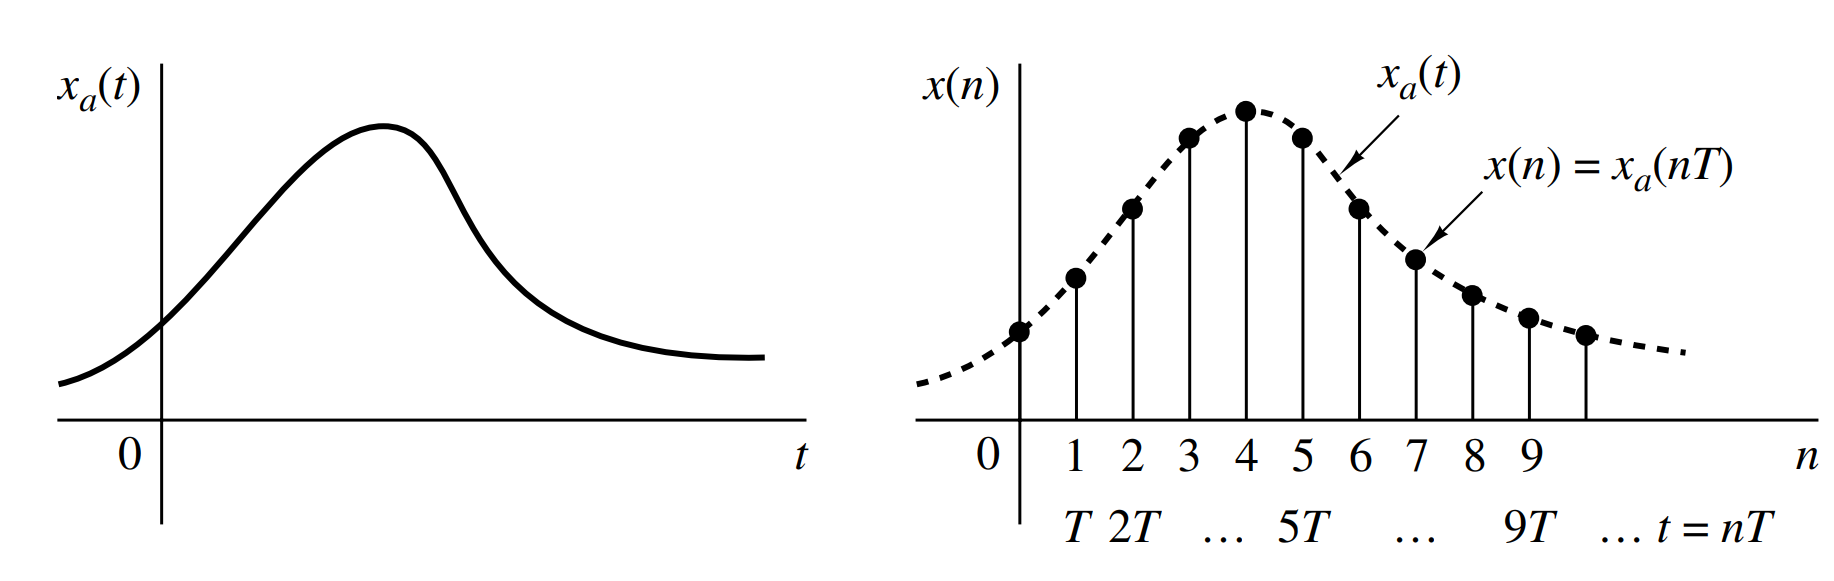
\includegraphics[scale=0.42]{img/periodic_sampling.png}
		\captionsetup{margin=2cm}
		\caption{ Periodic sampling of an analog signal. From \cite{proakis2006dimitris}.} 
		\label{fig:periodic_sampling}
	\end{center}
\end{figure}
\noindent At this point, it is important to point out how the sampling rate $F_s$ is selected in real \gls{dsp} applications. The acquisition of analog signals is typically driven by some prior knowledge about the characteristics of the signal to be sampled. In particular, this information concern the frequency content of general class of signals (e.g., the class of speech signals, the class of video signals, etc.), and they are generally available. For example, we know that human voice frequencies are, for the most part, below 3000 \gls{hz}. By knowing this information, appropriate sampling rate can be selected to avoid the problem commonly called \textit{aliasing}.\\
The latter occurs when the sampling rate is not sufficiently high to capture the higher frequencies of the original signal. The most common criterion to determine the sampling rate necessary to convert analog data to digital is given by the \textit{sampling theorem}, which was introduced by Nyquist (1928) and later popularized by Shannon (1949). This popular theorem states that it is possible to completely recover an analog signal $x_a(t)$ from its sample values if:
\begin{align}\label{eq:sampling_theorem}
	\begin{array}{c}
		F_s > 2\times F_{max}
	\end{array}
\end{align}
\noindent where $F_{max}$ is the largest frequency component in the analog signal. It is important to note that minimal sampling frequency that allows perfect reconstruction of a bandlimited signal from its samples, corresponds to $2\times F_{max}$. This sampling frequency is known as \textit{Nyquist rate}.\\ Thus, if the sampling rate is chosen according to the sampling theorem it is possible to avoid the problem of aliasing. A graphical example of the aliasing effect is given in Figure \ref{fig:aliasing}.

\begin{figure}[H]
	\begin{center}
		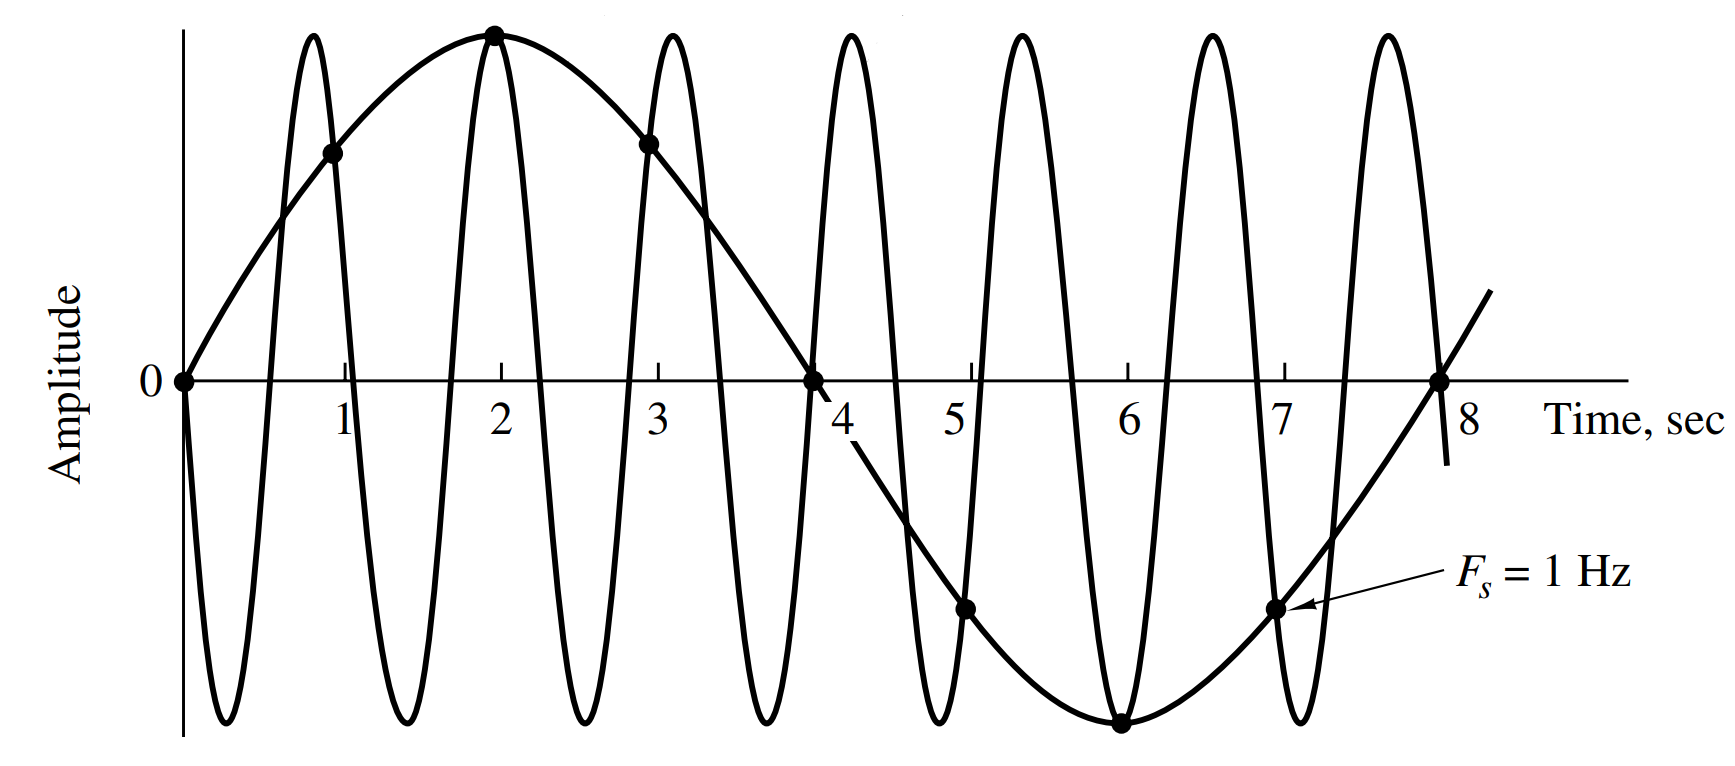
\includegraphics[scale=0.4]{img/aliasing.png}
		\captionsetup{margin=2cm}
		\caption{ Illustration of aliasing; the sampling frequency $F_{s} = 1$ \gls{hz} is not sufficiently high to unambiguously reconstruct the original sinusoid. From \cite{proakis2006dimitris}.} 
		\label{fig:aliasing}
	\end{center}
\end{figure}

\noindent Usually, after the sampling process, the quantization is performed. Briefly, quantization is the irreversible operation of converting a discrete-time continuous-amplitude signal into a digital one by expressing each sample value as a finite (instead of an infinite) number of digits. This results in signal distortion: it introduces the so called \textit{quantization error} which measures the difference between the quantized values and the actual sample ones. \\
Formally, let $x_{q}(n)$ denote the sequence of quantized samples at the output of the quantizer $Q[x(n)]$. Hence
\begin{align}\label{eq:quantizer}
	\begin{array}{c}
		x_{q}(n)=Q[x(n)]
	\end{array}
\end{align}

\noindent Then it is possible to define the quantization noise $e_{q}(n)$ as follows: 
\begin{equation}\label{eq:quant_noise}
	e_{q}(n)=x_{q}(n)-x(n)
\end{equation}
At this point, we can take an example to explain both the sampling and quantization processes more explicitly. First, consider the analog exponential signal
$$
x_a(t)=\left\{\begin{array}{ll}
	0.9^{t}, & t \geq 0 \\
	0, & t<0
\end{array}\right.
$$
\noindent Let $x(n) = 0.9^{n}, n \geq $ be the discrete-time signal obtained by the sampling process with $F_s = 1$ \gls{hz} (see Fig. \ref{fig:quantization} (a)). The resulting samples of $x(n)$ are shown in Table \ref{tab:quant}. As we can see, in this example, a complete description of the sampled signal requires $n$ significant digits. A precise description of each digit would be computationally heavy for most computers, and useless for many real applications. Thus, excess digits can be discarded by rounding the resulting number, as we can see in Figure \ref{fig:quantization} (b) and in Table \ref{tab:quant}. It is important to mention that the distance $\Delta$ between two successive quantized values is called \textit{quantization step}. 
\begin{figure}[]
	\begin{center}
		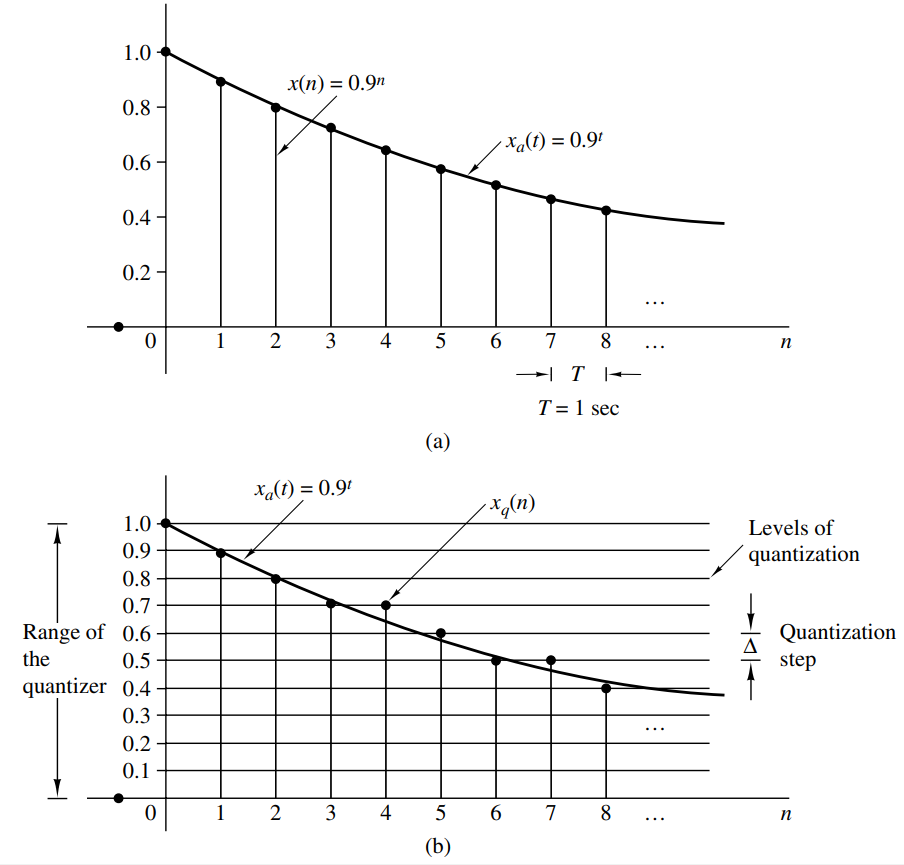
\includegraphics[scale=0.8]{img/quantization.png}
		\captionsetup{margin=2cm}
		\caption{Graphical example of quantization. From \cite{proakis2006dimitris}.} 
		\label{fig:quantization}
	\end{center}
\end{figure}

\begin{table}[]
	\begin{center}
		\begin{tabular}{clcl}
			\hline & $x(n)$ & $x_{q}(n)$ & $e_{q}(n)=x_{q}(n)-x(n)$ \\
			$n$ & Discrete-time signal & (Rounding) & Quantization Error \\
			\hline 0 & 1 & 1.0 & 0.0 \\
			1 & 0.9 & 0.9 & 0.0 \\
			2 & 0.81 & 0.8 & -0.01 \\
			3 & 0.72 & 0.7 & -0.029 \\
			4 & 0.6561 & 0.7 & 0.0439 \\
			5 & 0.59049 & 0.6 & 0.00951 \\
			6 & 0.531441 & 0.5 & -0.031441 \\
			7 & 0.4782969 & 0.5 & 0.0217031 \\
			8 & 0.43046721 & 0.4 & -0.03046721 \\
			9 & 0.387420489 & 0.4 & 0.012579511 \\
			\hline
		\end{tabular}
		\caption{Numerical illustration of quantization with one significant digit using rounding. From \cite{proakis2006dimitris}.}
		\label{tab:quant}
	\end{center}
\end{table}

\noindent As previously mentioned, the last step of \gls{ad} converters consists in the coding process. Thus, each sample is changed to an n bit code, such that each quantization level is assigned to a unique binary number.

\subsection{About Sinusoids}
Sinusoids are the building block of signal processing. As is described later in this chapter, all signals can be decomposed into constituent sinusoids of different frequencies using Fourier analysis. \\
Formally, it is possible to express a discrete-time sinusoidal signal as:
\begin{align} \label{eq:sinusoidal_signal}
	x(n) = A \sin(\omega n + \phi) = A \sin(2\pi fn + \phi) = A \sin(\frac{2\pi}{\tau}n + \phi), \qquad -\infty < n < \infty
\end{align}
\noindent The above definition introduces the following parameters \cite{christensen2019sound}:
\begin{itemize}
	\item The amplitude $A$, which scales the range of values of the sinusoid from  $[{-1},1]$ to  $[{-A},A]$.
	\item The frequency $\omega$ in radians per sample. Note that $\omega = 2 \pi f$, where $f$ is the frequency in cycles per sample. The frequency is inversely proportional to the period $\tau = \frac{1}{f}$, which measures the time the sinusoids takes to perform an entire cycle. 
	\item $\phi$ is the phase in radians. It can be thought of as a time-shift of the sinusoid.
\end{itemize}

\noindent It is important to note that sine and cosine are orthogonal waveform functions, i.e. they are out of phase by $\phi = \frac{\pi}{2}$. Therefore, from a terminological point of view, we refer to both cosine and sine functions as simply sinusoids. \\
A graphical example of a discrete-time sinusoid is given in Figure \ref{fig:sinusoidal_signal}.

\begin{figure}[H]
	\begin{center}
		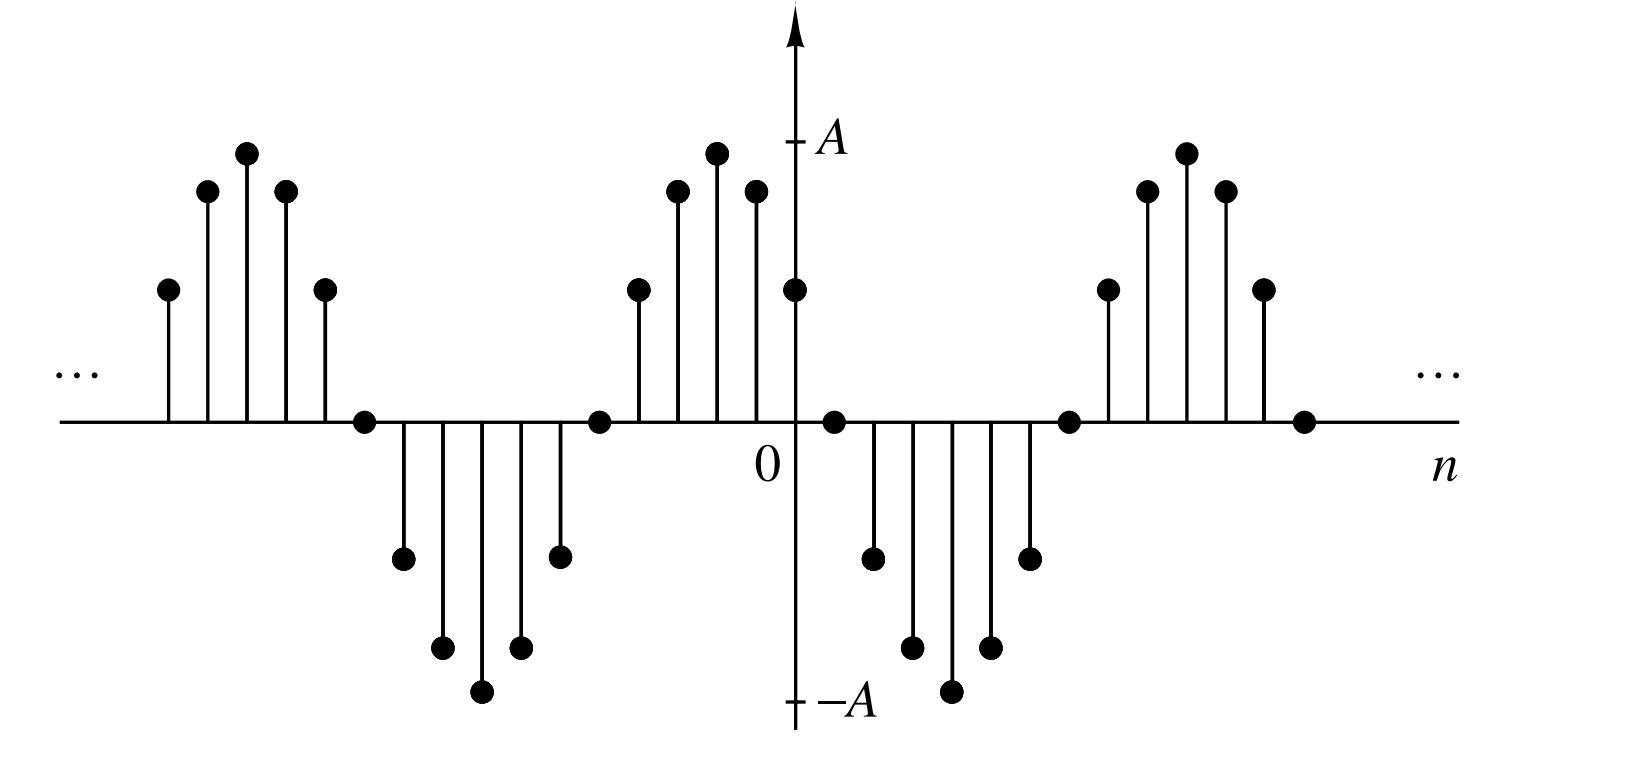
\includegraphics[scale=0.4]{img/sinusoidal_signal.png}
		\captionsetup{margin=2cm}
		\caption{Example of a discrete-time sinusoidal signal ($\omega = \frac{\pi}{6}$ and $\phi = \frac{\pi}{3}$). From \cite{proakis2006dimitris}.} 
		\label{fig:sinusoidal_signal}
	\end{center}
\end{figure}

\noindent It can be demonstrated  (see \cite{proakis2006dimitris}) that discrete-time sinusoids are characterized by the following properties:
\begin{itemize}
	\item A discrete-time sinusoid is periodic only if $f\in \mathbb{Q}$.
	\item Discrete-time sinusoids whose frequencies are separated by an integer multiple of 2$\pi$ are identical. From this property it follows that any sinusoid with a frequency $|\omega| > \pi$, or $|f| > \frac{1}{2}$, is an alias of a corresponding sequence resulting from a sinusoid with frequency $|\omega| < \pi$. For this reason, the range $0 \leq \omega \leq 2\pi$ or $-\pi \leq \omega \leq \pi$  ($0 \leq f \leq 1$, $-\frac{1}{2} \leq f \leq \frac{1}{2}$ ) is commonly defined as the \textit{fundamental range}.
	\item The highest rate of oscillation in a discrete-time sinusoid is attained when $|\omega| = \pi$ or, equivalently, $|f| = \frac{1}{2}$.
\end{itemize}

\subsubsection{Complex sinusoids}
\textit{Complex sinusoids}, (or \textit{complex exponentials}) are the building blocks of any real-world signal: as it is stated in Section \ref{fourier}, it is possible to decompose (or, at least, approximate) most signals of practical interest as a weighted sum of complex exponentials. Thus, it is important to introduce the class of these complex objects. \\
According to \cite{proakis2006dimitris}, we can define a complex exponential $x(n)$ as:
\begin{align}
	x(n) =  A e^{j(\omega n + \phi)} = A \cos(\omega n + \phi) + j A \sin(\omega n + \phi), \qquad -\infty < n < \infty
\end{align}
\noindent where $A$ is the amplitude and $j \in \mathbb{C}$ is the \textit{imaginary unit}. The link between exponential and trigonometric form of the above relation derives from the Euler identity, which is expressed as follows.
\begin{align}
e^{\pm j \theta}=\cos \theta \pm j \sin \theta
\end{align}

\subsection{Classification of Discrete-Time Signals}
The techniques used in \gls{dsp} depend heavily on the characteristics of the signal. Consequently, it is important to categorize signals based on their attributes. According to \cite{proakis2006dimitris}, important classes of discrete-time signals are the following.
\begin{itemize}
	\item \textit{Energy signals}. Consider a discrete-time signal $x(n)$, and let define the energy $E$ as:
	\begin{align}
		E =\sum_{n = -\infty}^{\infty} |x(n)|^2
	\end{align}
	If $E$ is finite, then $x(n)$ is an energy signal.
	\item \textit{Power signals}. The average power of $x(n)$ can be defined as:
	\begin{align}
	P=\lim _{N \rightarrow \infty} \frac{1}{2 N+1} \sum_{n=-N}^{N}|x(n)|^{2}
	\end{align}
	If $P$ is finite, then $x(n)$ is an energy signal.	Note that if $E$ is finite, $P = 0$, but if $E$ is infinite, $P$ may be either finite or infinite.
	\item \textit{Periodic signals}. A discrete-time signal $x(n)$ is periodi with period $N (N>0)$ if:
	\begin{align}
		x(n + N) = x(n) \qquad \forall n
	\end{align}
	The smallest value of $N$ for which this statement is true is called the fundamental period. It can be demonstrated (see \cite{proakis2006dimitris}) that  periodic signals are power signals. On the other hand, it is also worth noting that the energy of a periodic signal over a single period is finite if $x(n)$ takes on finite values over the period. 
	\item {Even and odd signals}. An even (or symmetric) signal $x(n)$ can be defined as a sequence with the following property:
	\begin{align}
		x(-n) = x(n)
	\end{align}
	On the other hand, a signal $x(n$) is called odd (or, equivalently, antisymmetric) if:
	\begin{align}
		x(-n) = -x(n)
	\end{align}
	Graphical examples of symmetric and antisymmetric signals are given, respectively, in Figure \ref{fig:evenodd} (a) and (b).
	\begin{figure}[H]
		\begin{center}
			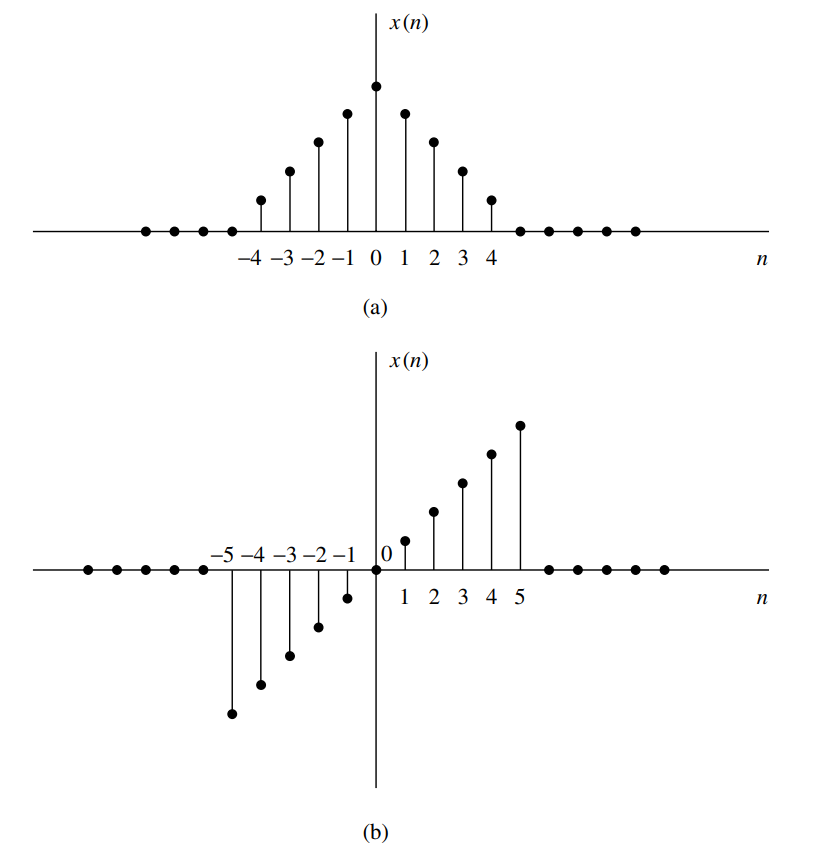
\includegraphics[scale=0.8]{img/evenodd.png}
			\captionsetup{margin=2cm}
			\caption{Example of even (a) and odd (b) signals. From \cite{proakis2006dimitris}.} 
			\label{fig:evenodd}
		\end{center}
	\end{figure}
\end{itemize}

\subsection{Spectral Analysis of Signals} \label{fourier}
Frequency analysis is a powerful tool that is widely used in a large variety of engineering and signal processing tasks. Briefly, the spectral representation aims to highlight how the energy is distributed across frequency components of the signal. Furthermore, the spectral representation is particularly suited for performing specific classes of operations, such as the convolution. \\
As previously mentioned, signals can be decomposed into a weighted sum of sinusoidal signal components (or complex exponentials). The decomposition techniques depend on the characteristic attributes of the specific signal. Indeed, there are frequency analysis tools that apply only to specific families of signals. In particular, periodic signals can be decomposed through \textit{Fourier series}; on the other hand, for the class of finite energy signals, the decomposition is called the \textit{Fourier transform}. \\
This section aims to explain the difference between these tools, by referring mainly to the book \cite{proakis2006dimitris}. Since this project deals only with digital signals, only definitions concerning discrete time-signals are discussed.
\subsubsection{Discrete-Time Fourier Series}
\textit{Fourier series} are used to decompose periodic sequences into a weighted sum of frequency components. Formally, suppose to have a discrete-time  periodic signal $x(n)$ with period $N$ such that $x(n)=x(n+N)\quad\forall n$. The Fourier series for that signal can be expressed as:
\begin{align}\label{Synthesis_eq_fs}
x(n)=\sum_{k=0}^{N-1} c_{k} s_{k}(n)
\end{align}
where {$c_k$} are the coefficients in the series representation and $s_{k}$ consists of $N$ harmonically related exponential functions, such that:
\begin{align} \label{harmonic}
s_k(n) = e^{j 2 \pi n \frac{k} {N}}, \qquad k=0,1, \ldots, N-1
\end{align}
The set defined in \ref{harmonic} is composed of periodic complex exponentials which share fundamental frequencies that are multiples of a single positive frequency term. It is noticeable that, from a terminological point of view, the sequence $s_k(n)$ is called the k-th \textit{harmonic} of $x(n)$.\\
The relationship \ref{Synthesis_eq_fs} is called \textit{Synthesis equation} or, equivalently, \gls{dtfs}. As for the Fourier coefficients $c_k$, they represents the amplitude and phase associated with the frequency component $s_k(n)$. In other words, these coefficients provide the description of the periodic signal $x(n)$ in the frequency domain. Their definition is provided by the \textit{Analysis equation} expressed in \ref{analysis_eq_fs}.
\begin{align}\label{analysis_eq_fs}
	c_{k}=\frac{1}{N} \sum_{n=0}^{N-1} x(n) e^{\frac{-j 2 \pi kn} {N}}, \qquad k=0,1, \ldots, N-1
\end{align}
\noindent Furthermore, it can be demonstrated that the spectrum of a periodic signal $x(n)$ with period $N$, is a periodic sequence with period $N$. Consequently, it is sufficient to observe any $N$ consecutive samples belonging to the signal in either time or frequency domain to provide its complete description.\\
Lastly, it is important to highlight that real periodic signals have interesting  symmetry properties. In particular, we know that for a real periodic signal, the spectral magnitude has an even symmetry property, such that: 
$$
|c_{-k}| = |c_k|
$$
As for the spectral phase, we know that:
$$
\measuredangle  c_{-k}= \measuredangle c_{k} \quad
$$
As a direct consequence of these properties, we can conclude that it is possible to specify the whole signal in the frequency domain by taking into account only $\lfloor \frac{N}{2} \rfloor$ consecutive values. 

\subsubsection{Discrete-Time Fourier Transform} %Discrete-Time Fourier Transform?
Aperiodic signals can be decomposed through Fourier Transforms. From the \gls{dsp} theory \cite{proakis2006dimitris} we know that, given a discrete-time signal $x(n)$ with finite energy, it is possible to represent its frequency content by the analysis equation \ref{eq:analysis dtft}.

\begin{align}\label{eq:analysis dtft}
X(\omega)=\sum_{n=-\infty}^{\infty} x(n) e^{-j \omega n} = \sum_{n=-\infty}^{\infty} x(n) e^{-j 2 \pi f n}
\end{align}

\noindent From a notational point of view, we can write that:
$$
x(n) \stackrel{\mathscr{F}}{\longleftrightarrow} X(\omega)
$$
to denote that $X(\omega)$ is the Fourier Transform of $x(n)$.\\
The formula in \ref{eq:analysis dtft} is also called \gls{dtft}. From a conceptual point of view, $X(\omega)$ represents the decomposition of $x(n)$ into its frequency components. \\
As in the case of \gls{dtfs}, we can define a synthesis equation (\ref{eq:synthesis dtft}) too.
\begin{align}\label{eq:synthesis dtft}
x(n)=\frac{1}{2 \pi} \int_{2 \pi} X(\omega) e^{j \omega n} d \omega = \frac{1}{2 \pi} \int_{-\pi}^{\pi} X(\omega) e^{j \omega n} d \omega 
\end{align}
\noindent It is worth noting that, since \gls{dtft} is a periodic function of the frequency variable $\omega$, it has a Fourier series expansion. Therefore, its Fourier coefficients are the values of $x(n)$. In other words, the synthesis equation just written can be considered as an analysis equation of the Fourier Series of $X(\omega)$. In fact, the \gls{dtft} of $x(n)$ results in a periodic signal, with period $2\pi$. This is demonstrated below.
$$
X(\omega+2\pi k) =\sum_{n=-\infty}^{\infty} x(n) e^{-j(\omega+2 \pi k) n} = \sum_{n=-\infty}^{\infty} x(n) e^{-j \omega n} e^{-j 2 \pi k n} =\sum_{n=-\infty}^{\infty} x(n) e^{-j \omega n}=X(\omega)
$$
\noindent Also in this case there are some important symmetry properties. It is possible to demonstrate (\cite{proakis2006dimitris}) that if $x(n)$ is real, then:
$$|X(-\omega)|=|X(\omega)| \qquad \text{(even symmetry)}
$$
$$
\measuredangle X(-\omega)=- \measuredangle X(\omega), \quad \text { (odd symmetry) }$$
From these relations, we can conclude that it is possible to determine the frequency content of $x(n)$ from the range of values $0 \leq f \leq \frac{1}{2}$ (or, equivalently $0 \leq \omega \leq \pi$) rather than $-\frac{1}{2} \leq f \leq \frac{1}{2}$ ($-\pi \leq \omega \leq \pi$). In other words, if we know $X(-\omega)$ in the range $0 \leq \omega \leq \pi$  we can calculate $X(-\omega)$ over $-\pi \leq \omega < 0$. Summing up, the whole description of a discrete-time real signal $x(n)$ in the frequency domain is determined over the continuous range of values $0 \leq \omega \leq \pi$.

\subsubsection{Discrete Fourier Transform}
The \gls{dft} is a computational tool that plays a very important role in a wide variety of \gls{dsp} applications, such as linear filtering, spectrum analysis and power frequency estimation. \\
As previously motivated, Fourier transform aims to perform frequency analysis of a signal by decomposing it into different frequency components. Such a spectral representation leads to a discrete function in the case of \gls{dtfs}, i.e. when the input $x(n)$ is periodic. On the other hand, \gls{dtft} on aperiodic signals is a continuous function of frequency; therefore, from a computational point of view, it is not a convenient representation of the signal spectrum. \\
For this reason, it is important to introduce \gls{dft}, which is a powerful tool for representing a signal in the spectral-domain in a computationally efficient manner. \\
Formally, if we have a signal $x(n)$ of length $N$, it is possible to represent its frequency content with the following equation.

\begin{align}\label{eq:dft}
	X(k) =\sum_{n=0}^{N-1} x(n) e^{-j \frac{2 \pi k n}{N}}, \quad k=0,1,2, \ldots, N-1 
\end{align}

\noindent Conceptually, the \gls{dft} relation in \ref{eq:dft} expresses the Fourier transform as a function of a $N$-length equally spaced set of discrete frequencies. Indeed, it is possible to observe that the function is parametrized by the use of a discrete variable $k \in [0,N] \subset \mathbb{Z}$ rather than a continuous one $\omega\in [0,2\pi] \subset \mathbb{R}$.\\
The signal $x(n)$ can be recovered from its frequency samples by the $N$-point \gls{idft} relation in \ref{eq:idft}. 
\begin{align}\label{eq:idft}
	x(n) = \frac{1}{N} \sum_{n=0}^{N-1} X(k) e^{j \frac{2 \pi k n}{N}}, \quad n=0,1,2, \ldots, N-1
\end{align}
\noindent It is possible to demonstrate (see \cite{proakis2006dimitris}) that if we have a finite-duration sequence $x(n)$ of length $N_{lim}<N$, then the \gls{idft} yields $x(n) = 0 \text{ for } N_{lim} \leq n \leq{N-1}$. Otherwise, if the sequence $x(n)$ is time-limited by a value $N_{lim}$ such that $N_{lim}>N$, the $N$-point \gls{idft} results in an aliased version of the original signal. \\
\gls{dft} is a powerful tool which has many properties. The objective of this section is not to provide an exhaustive analysis of these properties, for which we refer to excellent textbooks (such as \cite{proakis2006dimitris}); thus, our aim is to determine only the properties linked to real-valued sequences, since they are of fundamental importance for the developed models (as it is explained in Chapter \ref{chap:methods}).\\
In this regard, if $x(n)$ is real, then 
$$|X(N-k)|=|X(k)|$$ 
$$\angle X(N-k)=-\angle X(k)$$
Furthermore, it can be demonstrated that $x_{I}(n)= 0$.\\
Finally, it is important to mention that the importance of \gls{dft} and \gls{idft} operations is enhanced by the fact that there are computationally efficient procedures, such as the family of \gls{fft} algorithms, from which they can be performed. The computational complexity of these algorithms depends on whether or not the input signal has some specific attributes (such as the symmetry for real-valued sequences already described).

\subsection{Discrete-time Systems}
In \gls{dsp} terminology, each physical device or digital algorithm that performs some operation on signals is called \textit{system}. As previously motivated, when we work with data on a computer, time is discretized, so that each operation is performed on discrete-time signals. For this reason, we focus our attention on discrete-time systems, i.e. devices or algorithms that operate on a discrete-time signal. \\
Formally, we can define a system $S$ as a set of operations performed on the input (or \textit{excitation}) signal $x(n)$ to produce the output (or \textit{response}) signal $y(n)$. Figure \ref{fig:dtsystem} illustrates this definition. \\
\begin{figure}[]
	\begin{center}
		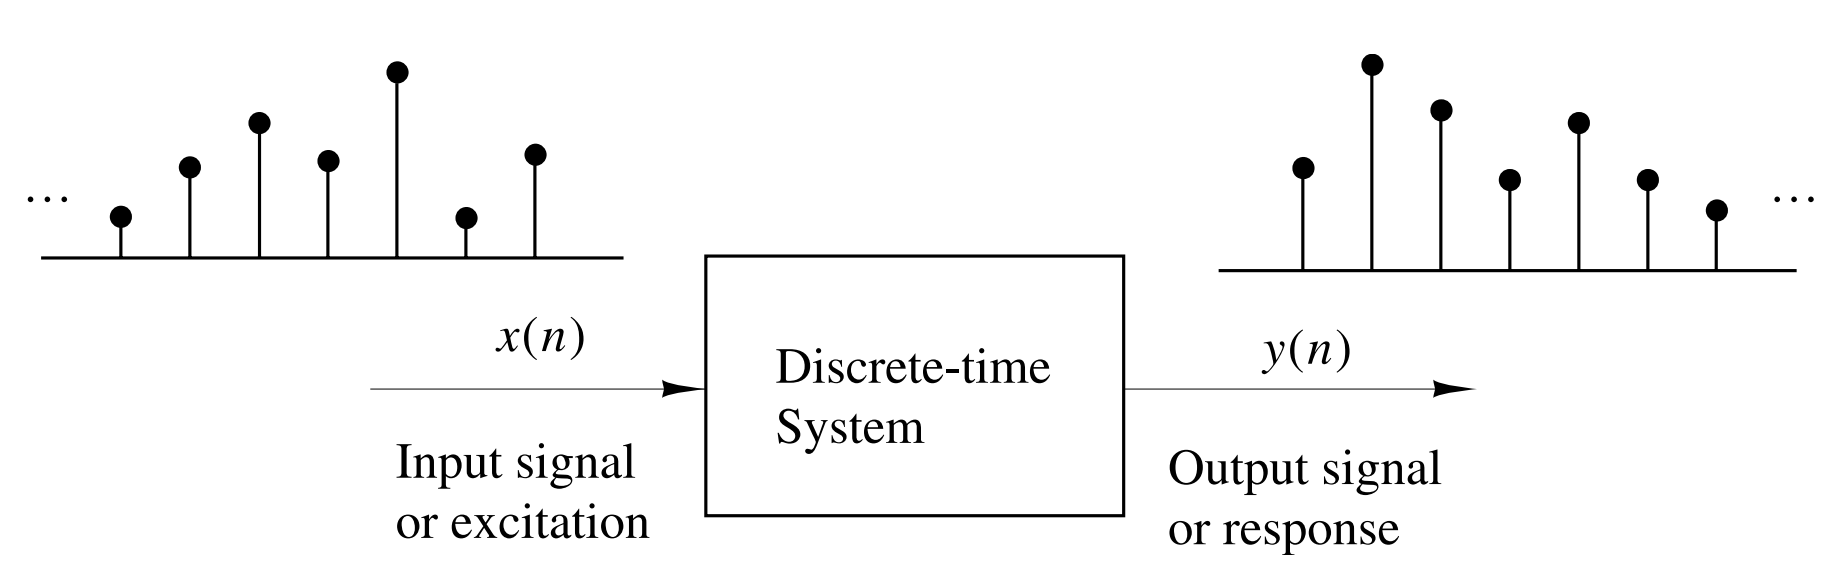
\includegraphics[scale=0.4]{img/dtsystem.png}
		\captionsetup{margin=2cm}
		\caption{Block diagram representation of a discrete-time system. From \cite{proakis2006dimitris}.} 
		\label{fig:dtsystem}
	\end{center}
\end{figure}
\noindent We can use equivalently the following two notations to express the transformation from $x(n)$ to $y(n)$ by the system $S$.
\begin{align}
	x(n) \xrightarrow{\text{S}} y(n)
	y(n) = S(x(n))
\end{align}
\noindent For our analysis purposes, as well as for providing a comprehensive
overview of the basic \gls{dsp} principles, it is important to classify systems according to their characteristics. In fact, the mathematical operations performed in this study are heavily dependent on the properties that the system satisfies. \\
According to \cite{proakis2006dimitris}, important classes of discrete-time systems are the following.

\begin{itemize}
	\item \textit{Time-invariant systems}. A system is called time-invariant if its input–output description $x(n) \xrightarrow{\text{S}} y(n)$ do not changes with time. Formally, let $x(n)$ be the input of a system $S$; if 
	$$y(n, k) = y(n - k) \quad \forall k$$
	where  $y(n, k) = S[x(n-k)]$, then $S$ is a time-invariant system. 
	\item \textit{Linear systems}. A system is said to be linear if it satisfies the principle of \textit{superposition}, which is formally described below. Given two arbitrary input sequences $x_1(n), x_2(n)$ and two arbitrary constants $a_1, a_2$ a system $S$ is linear if and only if:
	\begin{align}
		S[a_1x_1(n) + a_2x_2(n)] = a_1S[x_1(n)] + a_2S[x_2(n)] \qquad \forall x_1(n), x_2(n), a_1, a_2 
	\end{align}
	The above definition includes two important properties of linear systems: multiplicative and additive.
	\item \textit{Causal system}. A system called causal if its output depends only on present and past inputs	but does not depend on future ones. Formally, $S$ is causal if: 
	\begin{align}
		y(n) = F[x(n), x(n-1), x(n-2), ...]
	\end{align}
	where $F[.]$ is some arbitrary function. \\
	It is quite intuitive that causal system are at the basis of real-time \gls{dsp} applications, since the observation of input future values is  physically not possible. On the other hand, off-line processing often involves algorithms that perform \textit{non-causal} operations. A good example is provided by bi-directional \gls{rnn}s, which, for a given time step, process not only the past data elements in a given sequence, but also the future ones. 
\end{itemize}

\noindent Of particular importance for many \gls{dsp} applications is the class of \gls{lti} systems, whose response to an input sequence is determined by the \textit{convolution} operation. 


\subsubsection{Convolution}
Convolution is an important mathematical tool in both \gls{dsp} and \gls{dl} fields. In this section we introduce this operation from a theoretical perspective, while in paragraph \ref{cnns} its application in the context of neural networks is described. \\
In order to introduce the convolution, it is first important to define the \textit{unit sample sequence} (or \textit{unit impulse}), which corresponds to the most basic discrete-time signal. In particular, it is a signal that is zero everywhere, except at $n = 0$ where its value is unity. Formally:
\begin{align}
	\delta(n) = \begin{cases} 1 & \mbox{se } \mbox{ $n$ = 0} \\ 0 & \mbox{$ n\neq$ 0} \end{cases}  
\end{align}
\noindent Its graphical representation is provided in Fig. \ref{fig:unit}.
\begin{figure}[H]
	\begin{center}
		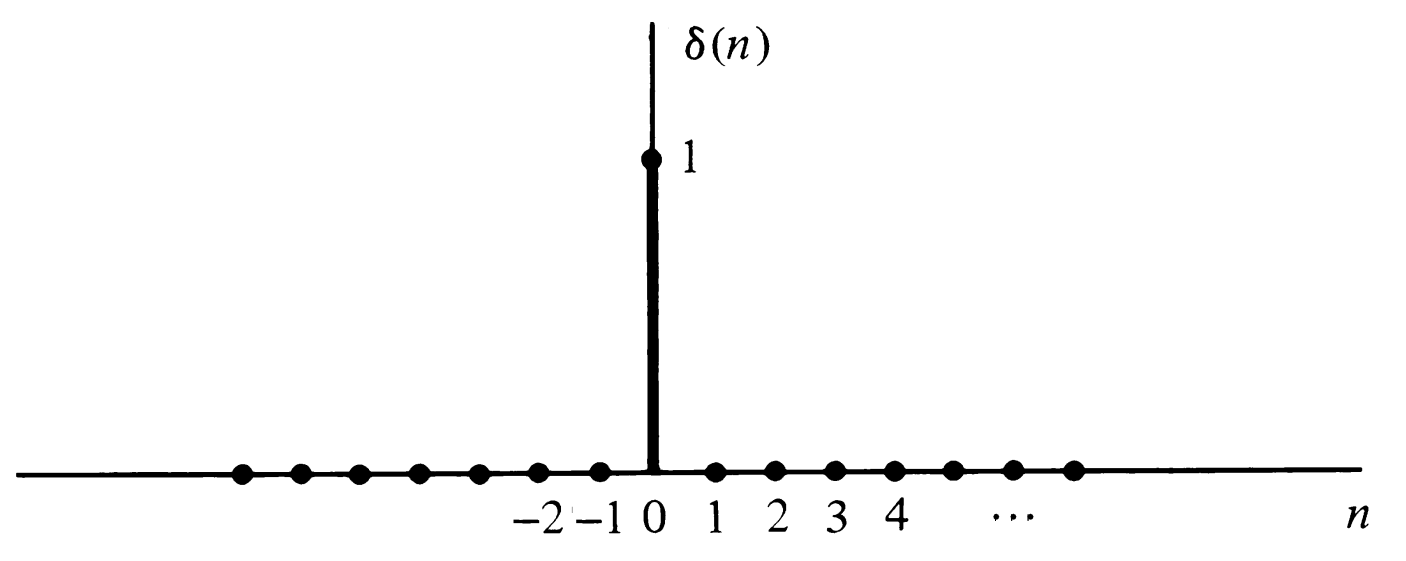
\includegraphics[scale=0.4]{img/unit.png}
		\captionsetup{margin=2cm}
		\caption{Graphical representation of
			the unit sample signal. From \cite{proakis2006dimitris}.} 
		\label{fig:unit}
	\end{center}
\end{figure}

\noindent At this point, it is possible to introduce the equation \ref{eq:decomposition_xn}, which expresses the decomposition of an arbitrary signal $x(n)$ into a weighted sum of shifted unit impulses.
\begin{align} \label{eq:decomposition_xn}
	x(n) =  \sum_{k = - \infty}^{\infty}x(k)\delta(n-k)
\end{align}
\noindent The importance of the relationship above expressed lies in the following considerations. \\
If we consider the response of a \gls{lti} system to $x(n)$ is the corresponding sum of weighted outputs, we obtain the expression \ref{eq:superp_summ}. 

\begin{align} \label{eq:superp_summ}
	y(n) = S[x(n)] = S\left[\sum_{k = - \infty}^{\infty}x(k)\delta(n-k)\right] =  \sum_{k = - \infty}^{\infty}x(k)S\left[\delta(n-k)\right]
\end{align}

\noindent Let now consider the unit sample signal $\delta(n)$ in a \gls{lti} system. We can denote as $h(n)$ the response of $S$ to this signal. Formally:
\begin{align} \label{eq:lti_resp}
	h(n) = S[\delta(n)]
\end{align}

\noindent The formula in \ref{eq:lti_resp} is of particular importance as it characterizes the system $S$: as stated in \cite{proakis2006dimitris}, \gls{lti} systems can be subdivided into FIR (finite-duration impulse response) and IIR (infinite-duration impulse response) depending on whether $h(n)$ has, respectively, finite or infinite duration. These concepts lie at the basis of the design of digital filters, for which we refer to the cited book.\\
Because of the system time-invariance property, it can be seen that:

\begin{align}
	h(n-k) = S[\delta(n-k)]
\end{align}

\noindent Consequently, the formula in \ref{eq:superp_summ} reduces to:
$$
	y(n) = \sum_{k = - \infty}^{\infty}x(k)h(n-k)
$$

\noindent which is called \textit{convolution sum} and can be better expressed with the following notation: 
\begin{align} \label{eq:conv_sum}
x(n) \circledast h(n) = y(n) = \sum_{k = - \infty}^{\infty}x(k)h(n-k)
\end{align}

\noindent The previous result (formula \ref{eq:conv_sum}) asserts that the response of an \gls{lti} system to a given input signal is obtained by \textit{convolving} the input sequence $x(n)$ with the system's response $y(n)$ to the unit impulse $h(n)$. \\
Furthermore, it is important to mention that, in \gls{dl} terminology (see \cite{goodfellow2016deep}), the first argument (in our definition, the function $x$) to the convolution is called \textit{input}, while the second argument ($h$) is called \textit{kernel}. Furthermore, the output $y$ is sometimes referred to as the \textit{feature map}. \\
The convolution operation has some important properties:

\begin{itemize}
	\item \textit{Commutative law}:
	\begin{align} 
		y(n) = x(n) \circledast h(n) = h(n) \circledast x(n) = \sum_{k = - \infty}^{\infty}x(k)h(n-k) = \sum_{k = - \infty}^{\infty}h(k)x(n-k)
	\end{align}
	\item \textit{Associative law}:
	\begin{align}
		[x(n) \circledast h_1(n)] \circledast h_2(n) = x(n) \circledast [h_1(n) \circledast h_2(n)]
	\end{align}
	\item \textit{Distributive law}:
	\begin{align}
		x(n) \circledast [h_1(n) + h_2(n)] = x(n) \circledast h_1(n) +  x(n) \circledast h_2(n)
	\end{align}
\end{itemize}
\noindent The convolution operation is an important tool even when we analyze the frequency response to \gls{lti} systems. In particular, we know from the so called \textit{convolution theorem} that convolution in the time domain is equivalent to multiplication in the frequency domain. \\
Formally, let $X(\omega), H(\omega), Y(\omega)$ be the spectra of, respectively, $x(n), h(n), y(n)$; then, the theorem asserts that:
\begin{align} \label{conv_theorem}
	y(n)=x(n) \circledast  h(n) \stackrel{\mathscr{F}}{\longleftrightarrow} Y(\omega)=X(\omega) H(\omega)
\end{align}
\noindent From this theorem we can conclude that convolution is an easier operation in the time domain rather than in the frequency one. \\


\section{Deep Learning}
The term \textit{artificial intelligence} is increasingly used in a variety of ways and behind it, there are many technologies. Rai et. al \cite{rai2019editor}, provide a quite comprehensive definition. "\gls{ai} is typically defined as the ability of a machine to perform cognitive functions that we associate with human minds, such as perceiving, reasoning, learning, interacting with the environment, problem solving, decision-making, and even demonstrating creativity". Although this definition is rather generic, it is possible to define, more specifically, the disciplines that belong to it. \\
Most of the time, researchers refers to the term \gls{ai} to indicate \gls{ml} algorithms. We can consider \gls{ml} as the discipline that extracts patterns of interest from data \cite{goodfellow2016deep}. \\
Mitchell \cite{mitchell1997machine} provides a quite formal definition of \gls{ml}: “A computer program is said to learn from experience E with respect to some class of tasks T and performance measure P, if its performance at tasks in T, as measured by P, improves with experience E”.\\
\gls{ml} is a very active research topic and it has many practical applications. Thus, the task T can range from medical diagnosis and community detection to antispam filtering and text categorization. However, many problems can be roughly categorized into two groups: classification (such as speaker identification) and regression (such as audio \gls{sr}). \\
In order to evaluate the performance of a \gls{ml} algorithm, a quantitative measure must be taken into account. Mitchell refers to this metric, which is always specific to the task T, as performance measure P. 
As for the learning experience E, \gls{ml} algorithms can be broadly categorized in two main classes: \textit{superivsed} and \textit{unsuperivsed}. Briefly, supervised learning aims to generate reliable predictions using labeled data. In other words, a supervised learning algorithm experiences a dataset on which each example is associated with a so called "ground truth", which represents the real output the model should be able to reproduce (or, at least, approximate). Audio super-resolution is a good example of supervised learning, since the goal is to learn a function that accurately maps the input \gls{lr} sequences to the corresponding \gls{hr} audio frames. \\
On the contrary, in unsupervised learning, the ground truth is not available. Indeed, the learning process focuses on useful properties of the dataset structure. Most of the time, the goal is to learn the entire probability distribution that generated the data. \\
It is possible to define a third category, i.e. \textit{semi-supervised learning}. According to Hady and Schwenker \cite{hady2013semi}, this approach aims to maximize the performance of a \gls{ml} model by integrating part or all of the available unlabeled data in its supervised learning process. \\
There are several different approaches in \gls{ml}, depending on the task and the data. On one hand, many problems can be tackled by designing a specific set of features to extract. The feature extraction step is very important, since the performance of the \gls{ml} algorithms are highly sensitive to the representation of the input data. \\
On the other hand, in some cases, it is not possible - or at least, is very difficult - to extract representative features for a specific task. For example, in the field of digital signal processing, descriptive variables such as energy, mean, variance, etc$\dots$ are not always sufficient to detect distinctive patterns of interest. In this case, we can use specific \gls{ml} approaches that can discover the right features to solve the problem by using raw data. This \textit{representation learning} approach often results in much better performance than can be obtained with hand-crafted feature extraction. Furthermore, representation learning is a less-time consuming approach since there is a minimal human intervention. \\
As for \textit{Deep Learning}, we can consider it as a \gls{ml} sub-field, in which the features are extracted through increasingly abstract hidden layers. \gls{dl} aims to estimate the desired mapping function by breaking it into a series of hidden mappings, each described by a different layer which provides a new representation of the input. \gls{dl} models result in complex computational graphs whose interpretability is often poor. \\
A schematic illustration of the newly introduced concepts is shown in Fig.\ref{fig:ai}.
\begin{figure}[H]
	\begin{center}
		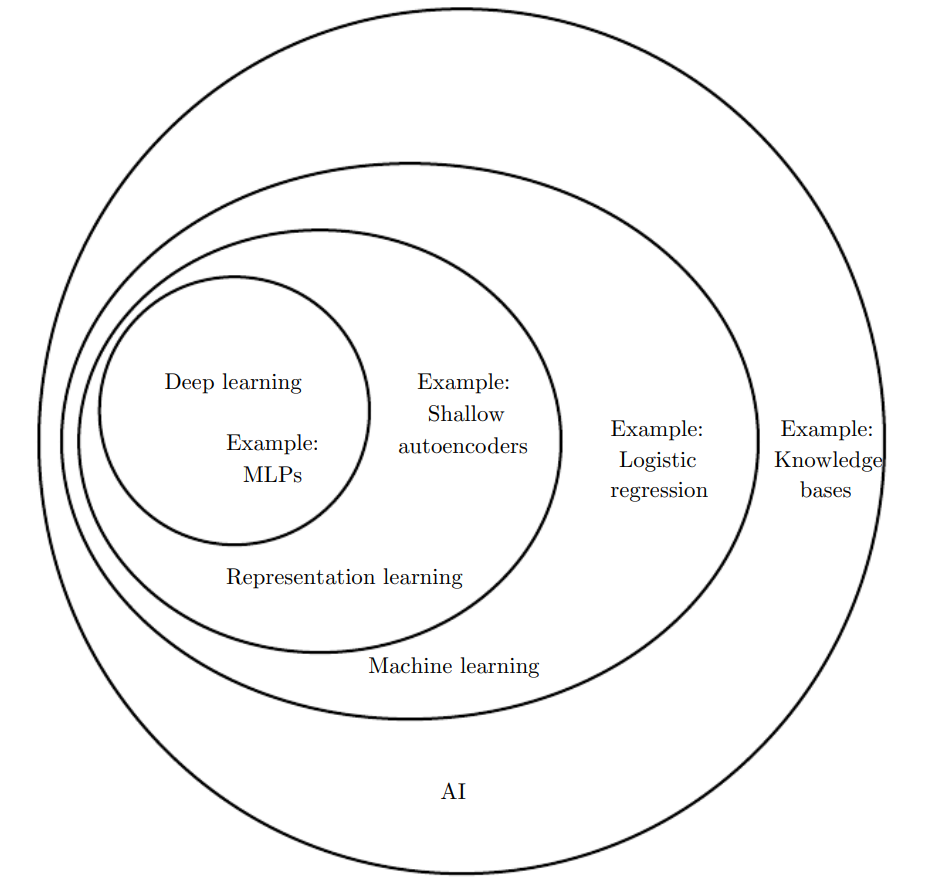
\includegraphics[scale=.7]{img/ai.png}
		\captionsetup{margin=2cm}
		\caption{A Venn diagram showing the conceptual location of \gls{dl},  \gls{ml} and \gls{ai} in the terms hierarchy. We can consider \gls{ai} as the term with the wider range of uses. Each section of the diagram includes an example of an \gls{ai} technology. From \cite{goodfellow2016deep}.}
		\label{fig:ai}
	\end{center}
\end{figure}
\noindent \gls{dl} is particularly effective when applied to large training sets, i.e. in high dimensional spaces with a large number of data points. Indeed, its use is perfectly suited for \gls{dsp} tasks, in which quite
a large amount of data is usually required. In this regard, it is noticeable that the popularity of deep-learning based approaches is largely due to their success in large-scale image classification tasks (see ImageNet \cite{ILSVRC15}). \\
There are many variants of deep-learning algorithms with different architectures and characteristics; some examples includes convolutional, generative and recurrent networks. The main objective of this section is to provide a broad description of these methodologies, trying to cover in a rather exhaustive way the main aspects that characterize them. A particular focus is given to convolutional and recurrent approaches, as they are of fundamental importance for the purposes of this work.

\subsection{The Learning Process} %o the learning process
As previously said, the task of Audio \gls{sr} belongs to the class of supervised learning problems; for this reason, we focus on the learning process, which is a central aspect that concerns this approach. \\
Briefly, supervised learning aims to learn a function $f_{\theta}$ that accurately maps input vectors $X$ to target labels $Y$. This formulation can be applied to a wide variety of problems; for example, we can see an audio \gls{sr} model as a mapping function of the form $f_{\theta}: X \rightarrow Y$ (see section \ref{problem_formulation}). \\
In order to measure how the function $f_{\theta}$ is accurate, we need to introduce the concept of \textit{objective function} also called \textit{loss function} or \textit{criterion}. We use these terms interchangeably though some researchers assign different meaning to some of these terms.\\
Formally, we can consider the criterion $L(\hat{y}, y)$ as a function which maps the model output $\hat{y}$ to a real number measuring the quality of the solution in terms of distance from the ground truth $y$. During the training phase, the parameters $\theta$ of the model are then set to optimize the loss. \\
Optimization in this case refers to the problem of minimizing (or, depending on the problem, maximizing) the objective function $L$ over the training samples. Proper solutions of the optimization problem can concern gradient-based methods; without going into that in detail, we only mention that these iterative optimization algorithms seeks to find the minimum (or the maximum) of a function by obtaining partial derivatives. Derivatives are important as they indicate on which direction each parameter of the model must be adjusted in order to reduce the error. \\
The most common optimization algorithms are Stochastic Gradient Descent \cite{kiefer1952stochastic}, Adam \cite{kingma2014adam}, Nadam \cite{dozat2016incorporating}, $\dots$ In all cases, the main idea is that, at each iteration, the loss function must be decreased by moving it in the direction of the negative gradient. The model parameters are then adjusted through the backpropagation algorithm \cite{amari1993backpropagation}. The convergence toward the minimum of the objective function model ~-~ and the speed of this convergence ~-~ depends upon the \textit{learning rate}, a positive scalar value. \\
For more details about these interesting aspects, as well as for a formal statement, we refer to the book "Deep Learning" \cite{goodfellow2016deep} by Goodfellow, Bengio and Courville. \\
As for loss functions, we mention, as typical examples, Negative Log-Likelihood, Cross-Entropy and \gls{mse}; the choice of which one to use is strongly influenced by the nature of problem. \\
A key aspects of optimization in \gls{dl} problems, is that loss functions are not necessarily convex. Ideally, we would obtain the global minimum, but this is not always possible, since there are multiple local minima and plateaus. For this reason, suboptimal solutions are generally accepted, as long as they correspond to significantly low values of the cost function.
\\
The main challenge of \gls{dl} (or, more generally, \gls{ml}) problems is that we must produce good predictions on unseen data. Indeed, according to \cite{goodfellow2016deep}, we can determine how well an algorithm performs by looking for its ability to both obtain a sufficiently low error value on the training set and minimize the gap between training and test error. Both abilities are of fundamental importance to avoid \textit{underfitting} and \textit{overfitting} problems. In particular, when the model is not able to make the training error small, we say it underfits. On the other hand, overfitting occurs when we measure a large gap between training and test error. The desired behavior occurs when the algorithm succeeds in learning the data distribution, providing good performance on the training set and, at the same time, can \textit{generalize} well on previously unobserved instances. \\
Underfitting and overfitting can be defined as function of two different sources of error: \textit{bias} and \textit{variance}. The former is a measure of the expected deviation of the estimator relative to the true value. From a statistical point of view, although unbiased estimators are desirable, since they have important properties, they are not always the best estimators. At the same time, a high bias can cause the underfitting. \\
On the other hand, variance measures the variability of the estimator about the expected value. If the model gets too sensitive to small variations of the data points during the learning phase, the generalisation capability can then be very poor (overfitting). \\
Therefore, when training a \gls{dl} model, it is important to take into account these aspects, as we aim to simultaneously minimize these two sources of error. This conflict is known in literature as "bias-variance trade-off". Figure \ref{fig:underoverfitting} provides a graphical representation of this problem. \\
\begin{figure}[H]
	\begin{center}
		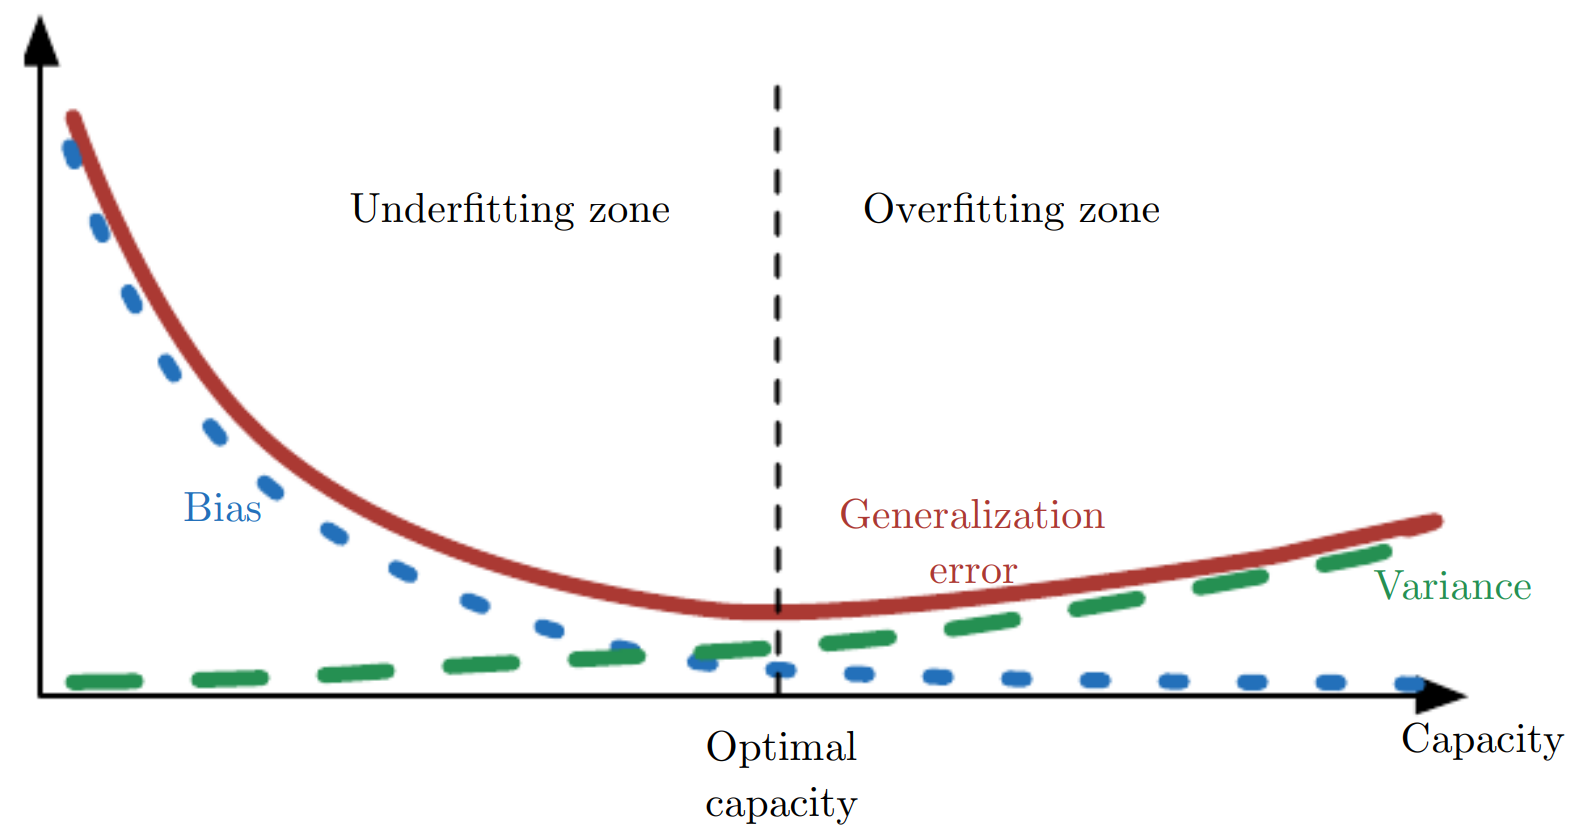
\includegraphics[scale=.4]{img/underoverfitting.png}
		\captionsetup{margin=2cm}
		\caption{Bias and Variance trade-off. As the capacity (complexity) of the model increases (x-axis), bias (dotted) tends to decrease and variance (dashed) tends to increase. The optimal capacity occurs when both bias and variance errors are minimized. From \cite{goodfellow2016deep}.}
		\label{fig:underoverfitting}
	\end{center}
\end{figure}
\noindent When overfitting occurs, it is possible to adopt regularization strategies with the specific aim to reduce the variance. Such techniques may vary according to the algorithms and the structure of the problem; to summarize, we only take into account regularization strategies for neural networks. \\
According to \cite{goodfellow2016deep}, we can refer to regularization as “any modification we make to a learning algorithm that is intended to reduce its generalization error but not its training error.”  \\
Typical examples of regularization techniques concern L1 and L2, which can be theoretically applied to any algorithm as they add parameter norm-based penalty to the objective function. \\
Another common strategy, especially in \gls{dsp} applications, is the so called "data augmentation". This is particularly suited when the dataset is small, as it allows the generation of additional and more diversified data points through certain transformations conducted upon original instances. Data augmentation is the easiest and cheapest way to increase the amount of training samples; however, the acquisition of new data, when possible, is preferable.  The correct transformation to apply highly dependent on the particular application. In Figure \ref{fig:data_aug} it is possible to see different ways of doing augmentation on images. \\
\begin{figure}[H]
	\begin{center}
		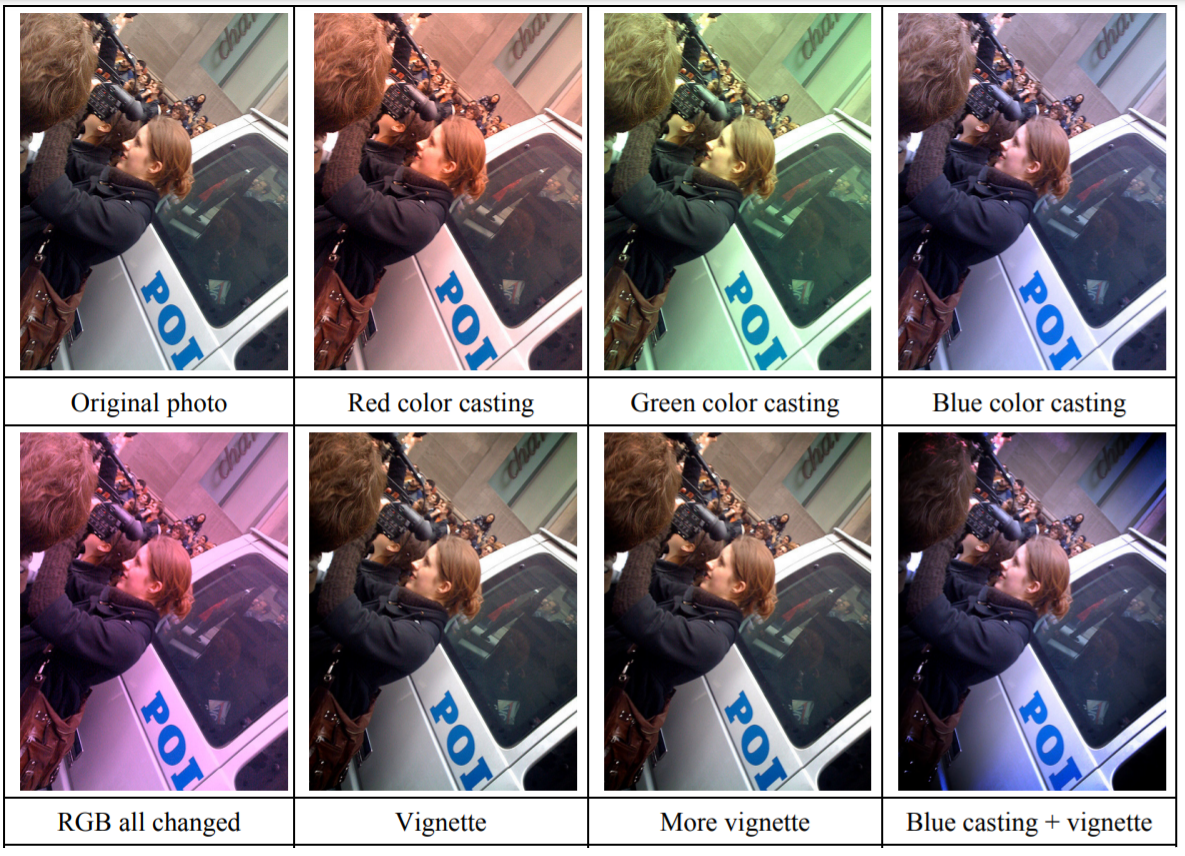
\includegraphics[scale=.55]{img/data_aug.png}
		\captionsetup{margin=2cm}
		\caption{Examples of color augmentations tested by Wu et al \cite{wu2015deep}.}
		\label{fig:data_aug}
	\end{center}
\end{figure}
\noindent Particularly worthy of mention are \textit{dropout}  \cite{srivastava2014dropout} and \textit{early stopping}, as they are two of the most used regularization strategies in \gls{dl} (and are both used in this project). \\
The former is a popular method to improve generalization by stochastically “dropping out” units during training to prevent their co-adaptation.\\
As for early stopping, briefly, it is based on choosing when to stop training a \gls{dl} model. The interruption criterion can vary wildly depending on the application; however, it is fair to say that it mostly depends on the loss on a validation set. An intuitive way of thinking about early stopping in \gls{dl} setting is to consider it as a hyperparameter selection method, where training time is the hyperparameter to be optimized.

\subsection{Convolutional Neural Networks} \label{cnns}
As previously motivated, \gls{cnn}s are an essential tool when facing \gls{dsp} problems and, for this reason, they are introduced in this section. \gls{cnn}s have revolutionized both the \gls{dsp} and the \gls{dl} fields, to the point that several \gls{dl}-based applications performs even better than human. \\ \gls{cnn} and, more generally \gls{dl}, came to mainstream popularity when Krizhevsky et al. \cite{krizhevsky2012imagenet} won the 2012 ImageNet Large-Scale Visual Recognition Challenge (ILSVRC \cite{ILSVRC15}) with a convolutional architecture called AlexNet. \\
The name Convolutional Neural Networks indicates that the system employs, in at least one of its layers, the convolution operation, which is previously introduced. Unlike in audio processing applications, where the convolution is generally applied only to one-dimensional signals, in \gls{dl} systems, usually this operation takes place between tensors, i.e. multidimensional vectors. Furthermore, in many \gls{dl} architectures the operation used in a \gls{cnn} does not correspond precisely to the traditional convolution: indeed, there are several variants such as the one defined in paragraph \ref{dilated_conv}. \\
\begin{figure}[H]
	\begin{center}
		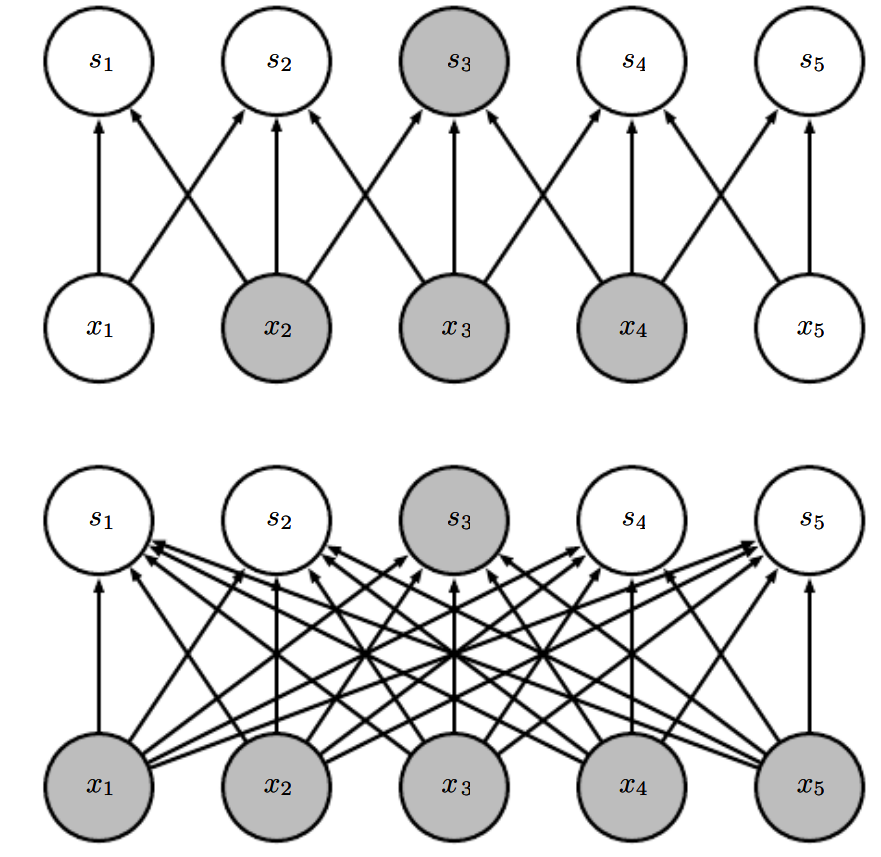
\includegraphics[scale=.5]{img/sparse_interactions.png}
		\captionsetup{margin=2cm}
		\caption{Graphical representation of the connections between input and output units in both convolutional and fully connected approaches. \textit{Top:} When we use \gls{cnn} layers with a kernel of width 3, the connectivity is sparse such that each output unit is affected only by 3 input units. \textit{Bottom:} In fully connected layers each output unit is formed by matrix multiplication, so that all of the inputs affect the highlighted $s_3$.
			From \cite{goodfellow2016deep}.}
		\label{fig:sparse_interactions}
	\end{center}
\end{figure}
\noindent One of the main advantages of \gls{cnn}s over traditional fully connected layers is that they allows to reduce the memory requirements by limiting the number of connections between input and output units. Thus, while in fully-connected layers forward propagation as well as backpropagation are expressed as matrix multiplications, \gls{cnn} layers use convolution which connects input and output units sparsely. This \textit{sparse connectivity} (also referred to as \textit{sparse interactions}) in convolutional networks reduces the computational complexity since the output computation requires fewer operations. In particular, the higher the \textit{receptive filed} of a convolutional layer is, the higher is the number of parameters, i.e. the memory requirements. A graphical illustration of the sparse interactions between input and output units is given in Figure \ref{fig:sparse_interactions}. \\
Even if direct connections in a convolutional net are very sparse, units in the higher layers can indirectly interact with a larger portion of the input. In other words, deeper layers receive generally more global information since the receptive field of the units in the higher layers is larger than the one of the units in the shallow layers. Furthermore, this effect is more pronounced if the system includes operations like \textit{pooling} (see the book \cite{goodfellow2016deep}). A graphical example of this intuitive concept is given in Figure \ref{fig:deeperlayers}. \\
\begin{figure}[H]
	\begin{center}
		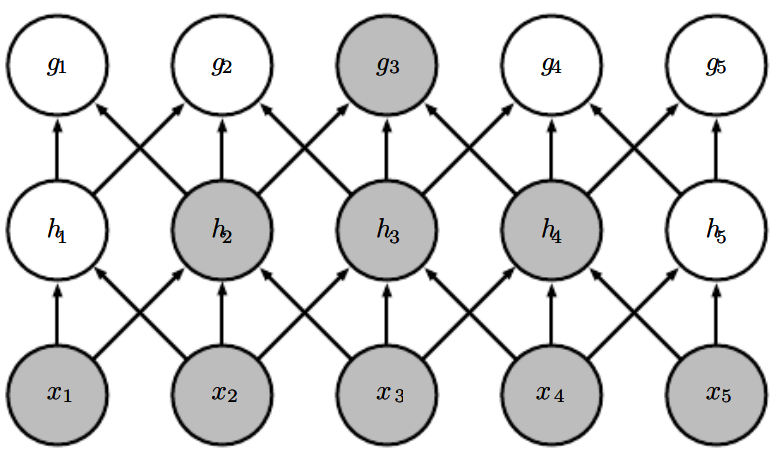
\includegraphics[scale=.5]{img/deeperlayers.png}
		\captionsetup{margin=2cm}
		\caption{Deeper layers can indirectly interact with a larger portion of the input.
From \cite{goodfellow2016deep}.}
		\label{fig:deeperlayers}
	\end{center}
\end{figure}
\noindent As previously motivated, deep convolutional networks are particularly suitable to capture complicated non-linear interactions between data points. The learning process leads to the creation of deep latent variables, which are quite difficult for a human to interpret. Because of this “black-box” nature, \gls{dl} models suffer from providing meaningful interpretations of their results. For this reason, the interpretation of deep networks is a very active research area, and many works in literature aims to discover what a \gls{cnn} really learns from data.\\
An interesting paper is that of Zeiler and Fergus \cite{zeiler2014visualizing} who works on images. They demonstrate that different layers of a \gls{cnn} respond distinctively to specific aspects of images. In particular, they discover that early hidden layers detect low-level features such as edges, corners and shapes, while deeper layers extract more abstract (high-level) information, such as categories or objects. Figure \ref{fig:cnnviz} provides a graphical example of this information hierarchy during the \gls{cnn} learning process.\\
\begin{figure}[H]
	\begin{center}
		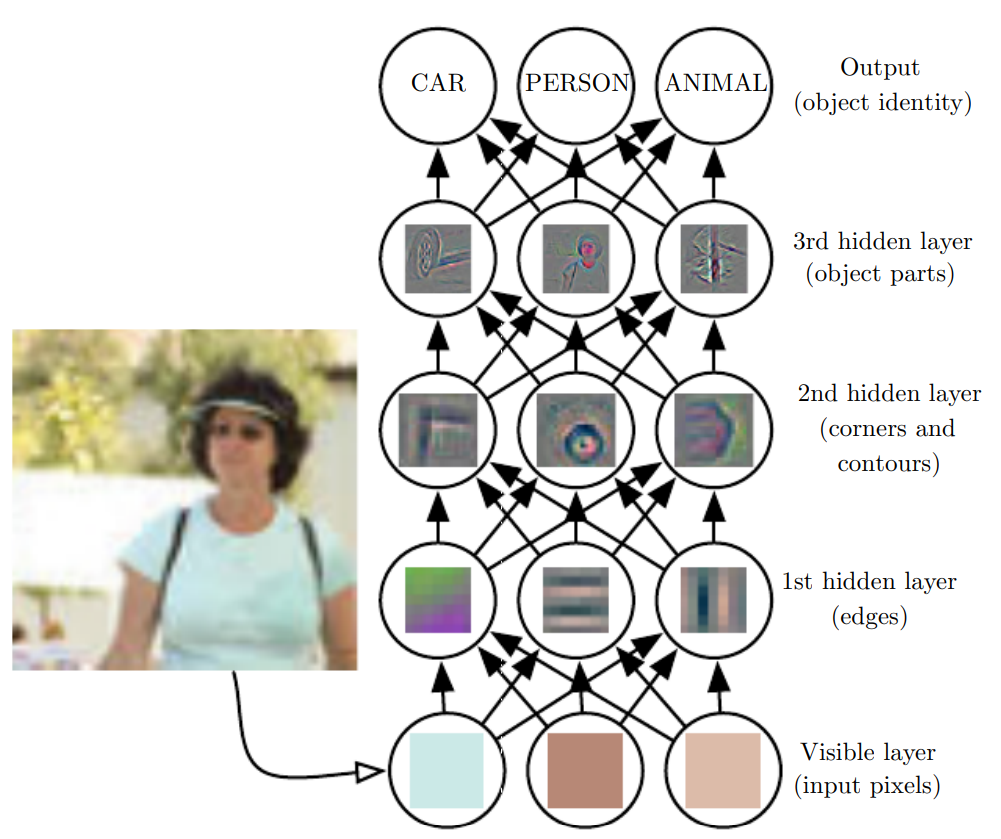
\includegraphics[scale=.7]{img/cnnviz.png}
		\captionsetup{margin=2cm}
		\caption{A convolutional neural network extracts increasingly abstract
			features from an image. From \cite{goodfellow2016deep}.}
		\label{fig:cnnviz}
	\end{center}
\end{figure}
\subsection{Recurrent Neural Networks}
In a traditional neural network we assume that input and output data do not follow a specific order; in other words, the implicit assumption is that data points are independent of each other. Although this assumption is valid in many problem settings, it is extremely limiting in others. For example, if we want to analyze historical data representing the global earth temperature, we have to take into account the implicit time axis between each observation. In speech processing too, data points are dependent of each other and this leads to the need for an appropriate sequential modelling. \\
Recurrent neural network approaches arise from this need: according to \cite{goodfellow2016deep}, much as a \gls{cnn} is particularly suited for processing data that have a grid pattern, such as images, a \gls{rnn} is specialized for processing time series, or, more generally, sequential data. An intuitive way to think about \gls{rnn}s is that they have a sort of "memory" which stores relevant information about what they have processed so far. \\
More specifically, \gls{rnn}s define recurrence relations between data points by introducing cycles in their computational graph to efficiently model this sequential influence. \\
The basic idea behind recurrent approaches is that, at each time step, an interaction takes place through hidden recurrent connections. This interaction, which involves a cycle in the graph computation, is graphically represented by a black square in Figure \ref{fig:rnn_graph}. \\
\begin{figure}[H]
	\begin{center}
		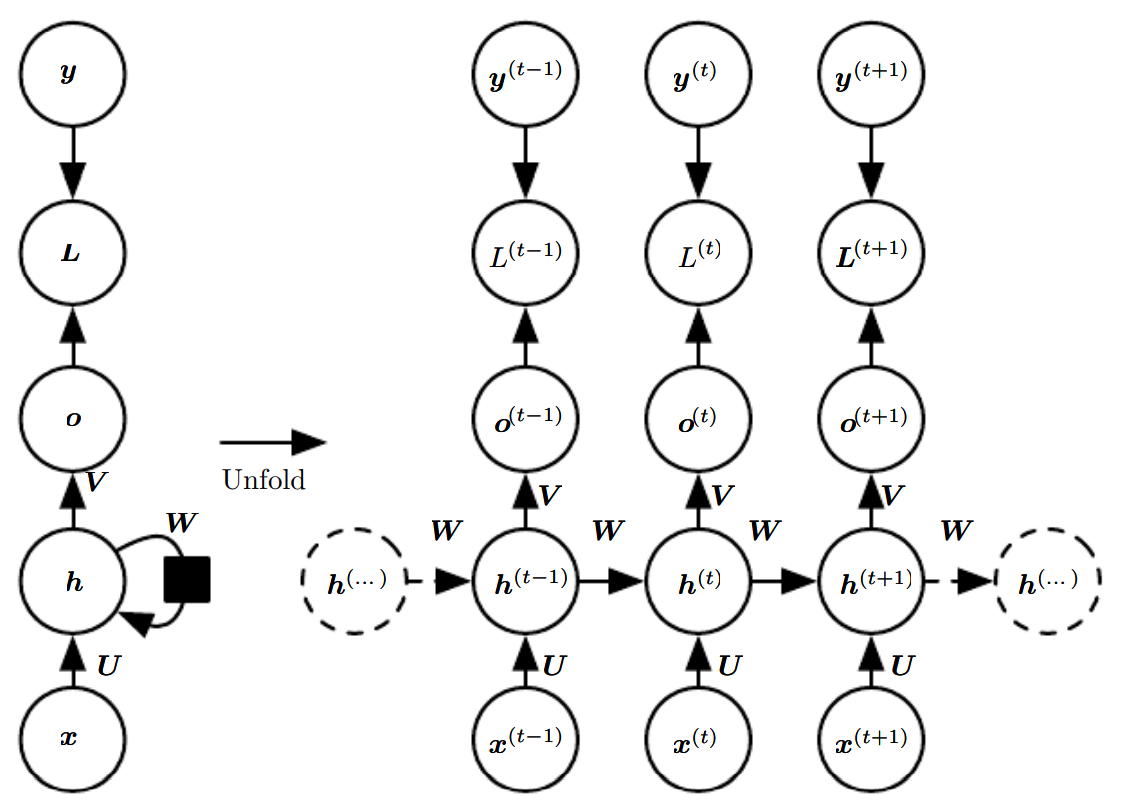
\includegraphics[scale=.58]{img/rnn_graph.png}
		\captionsetup{margin=2cm}
		\caption{"The computational graph to compute the training loss of a recurrent network that maps an input sequence of \textbf{x} values to a corresponding sequence of output \textbf{o} values.	A loss \textbf{L} measures how far each \textbf{o} is from the corresponding training target \textbf{y}. When using softmax outputs, we assume \textbf{o} is the unnormalized log probabilities. The loss \textbf{L} internally computes \textbf{$\hat{y}$} = softmax(\textbf{o}) and compares this to the target \textbf{y}. The \gls{rnn} has input to hidden connections parametrized by a weight matrix \textbf{U}, hidden-to-hidden recurrent connections parametrized by a weight matrix \textbf{W}, and hidden-to-output connections parametrized by a weight matrix \textbf{V}". \textit{Left:} Circuit diagram representation. \textit{Right:} The same \gls{rnn} seen as an unfolded computational graph. From \cite{goodfellow2016deep}.}
		\label{fig:rnn_graph}
	\end{center}
\end{figure}
\noindent Figure \ref{fig:rnn_graph} illustrates a simple \gls{rnn} that processes the information from the input \textbf{x} by incorporating it into the state \textbf{h} that is passed forward through time. \\
It is noticeable that this architecture aims to produce an output at each time step and has recurrent connections between hidden units. Although this is a common schema, it may not be the rule. Indeed, depending on the task, it might be reasonable to adopt other architectural configurations. For example, when working on a speaker identification task, we aim to obtain the final output after the whole input recording is processed, not after each audio sample. In this case we need a \gls{rnn} that reads an entire sequence and produces a single output, such as the one illustrated in Figure \ref{fig:rnn_single_output}. \\
\begin{figure}[H]
	\begin{center}
		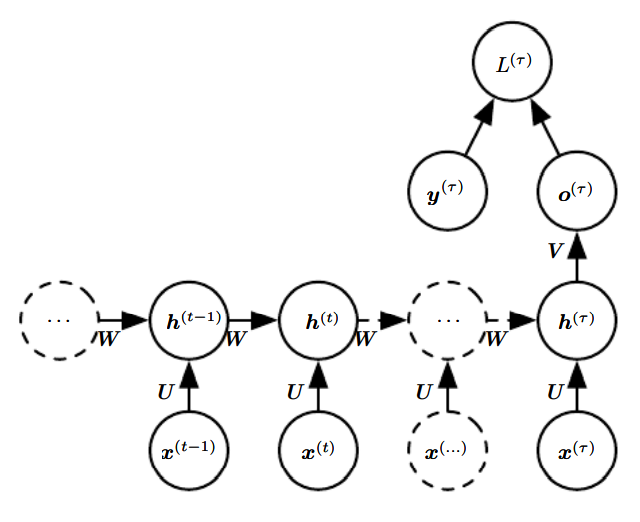
\includegraphics[scale=.75]{img/rnn_single_output.png}
		\captionsetup{margin=2cm}
		\caption{Time-unfolded \gls{rnn} with a single output at the end of the sequence. From \cite{goodfellow2016deep}.}
		\label{fig:rnn_single_output}
	\end{center}
\end{figure}
\noindent It is important to mention that recurrent networks are trained through the Backpropagation Through Time algorithm (\cite{rumelhart1985learning}, \cite{werbos1990backpropagation}), which computes the gradient of model error with respect to its weights. \\
Common problems in recurrent \gls{dl} approaches are the ones of \textit{vanishing} and \textit{exploding} gradients. Especially traditional \gls{rnn}s suffer from it: if the gradient tends to be very close to zero in the training process, the network weight correction vanishes and, consequently, the backpropagation through time fails. \\
One possible solution to reduce the effect of vanishing gradients would be to adopt \textit{gated} \gls{rnn}s architectures. These special sequence models include \gls{lstm}\cite{hochreiter1997long} and \gls{gru}\cite{chung2014empirical}. Without going into too much detail, gated \gls{rnn}s are based on the idea of creating few trainable gates (paths) to select the most important information to memorize through time. These pieces of informations are then propagated by connection weights that may change at every time step. For a more formal and comprehensive description of these recurrent approaches we encourage to consider deep learning textbooks, such as \cite{goodfellow2016deep}. 